\documentclass{beamer}
\usepackage[utf8]{inputenc}
\usepackage{graphicx}
\usetheme{Warsaw}  %% Themenwahl
\usepackage{csvsimple}
\usepackage{ngerman}
\usepackage[utf8]{inputenc}
\usepackage{listings}
\usepackage{amsmath}
\usepackage{hyperref}
\usepackage{amssymb}
% wegen deutschen Umlauten
%\usepackage[ansinew]{inputenc}
%Grafiken einbinden
\usepackage[ngerman]{babel}

\title{Data Mining}
\subtitle{ Itemset Mining}
\author{Jonas Grab, Christian Ley, Christian Stricker}
\date{\today}
	
\begin{document}
\frame{\titlepage}
\frame{\tableofcontents[currentsection]}



\section{Grundidee}
\begin{frame} %%Eine Folie
  \frametitle{Grundidee} %%Folientitel

  		Lesen Datensatz ein\\
  		Bestimme einelementige Tupel die freq sind\\
  		Solange prevFreq nicht leer:\\
  		\hspace{0.7cm}Baue aus prevFreq alle canidates\\
  		\hspace{0.7cm}Überprüfe alle canidates, ob alle deren Subtupel freq sind\\
  		\hspace{0.7cm}Prüfe welche restlichen canidates  wirklich freq sind
\end{frame}



\section{Optimierung 1}
\begin{frame} %%Eine Folie
	\frametitle{Optimierung 1} %%Folientitel
	\begin{itemize}
		\item Codiere jede Zeile vom input binär:\\
			\hspace{0.7cm}$1,0,1,1 => 1101_2 = 13_{10}$\\
			\hspace{0.7cm}$0,0,1,1 => 1100_2 = 12_{10}$
		\item Freq-Tupel auch binär codieren:\\
			\hspace{0.7cm} Freq Tupel $\{3\}$ in binär: $0100_2 = 4_{10}$\\
			\hspace{0.7cm} Freq Tupel $\{1,4,5\}$ in binär: $11001_2 = 25_{10}$
		\item Binäre Operationen wie $'or', 'and', 'equal'$ auf einzelnen Zahlen schneller als bei Arrays/Listen
	\end{itemize}
\end{frame}


\section{Optimierung 2}
\begin{frame} %%Eine Folie
	\frametitle{Optimierung 2} %%Folientitel
		\begin{itemize}
			\item Bedingung Freq-Tupel: alle seine Sub-Tupel müssen freq sein
			\item Original: Erzeuge und prüfe alle Sub-Tupel 
			\item Verbesserung: Wie oft wurde next-freq-Tupel aus den prev-freq-Tupel erzeugt:\\
				\hspace{0.7cm}Bsp.: $\{1,2,3\} = 111_2$ muss 3 mal aus den prev-Tupeln: \\
				\hspace{1.0cm}${011_2=\{1,2\}, 101_2=\{1,3\}, 110_2=\{2,3\}}$ erzeugt\\
				\hspace{1.0cm}werden
				\hspace{0.7cm} 
			\item Für Iteration k müssen k-mal das next-freq-Tupel erzeugt werden
		\end{itemize}
\end{frame}


\section{Border}
\begin{frame} %%Eine Folie
	\frametitle{Border} %%Folientitel
		\begin{itemize}
			\item Borders sind eine kürzere Darstellung für alle Frequent Itemsets:
			\item negative Border: die ersten Itemsets, die nicht mehr frequent sind
			\item positive Border: die letzten Sets die noch frequent sind
			\item Darstellung viel kleiner (Speicherbedarf)
			\item Berechnung gleich aufwendig
		\end{itemize}
\end{frame}

\section{Sets}
\begin{frame} %%Eine Folie
	\frametitle{Sets} %%Folientitel
		\begin{itemize}
			\item Free-Sets: Alle Vorherigen Subsets sind häufiger:
				\begin{itemize}
					\item Wenn Tupel freq ist, überprüfe Häufigkeit zu seinen Subsets
				\end{itemize}
		\end{itemize}
		\centering
		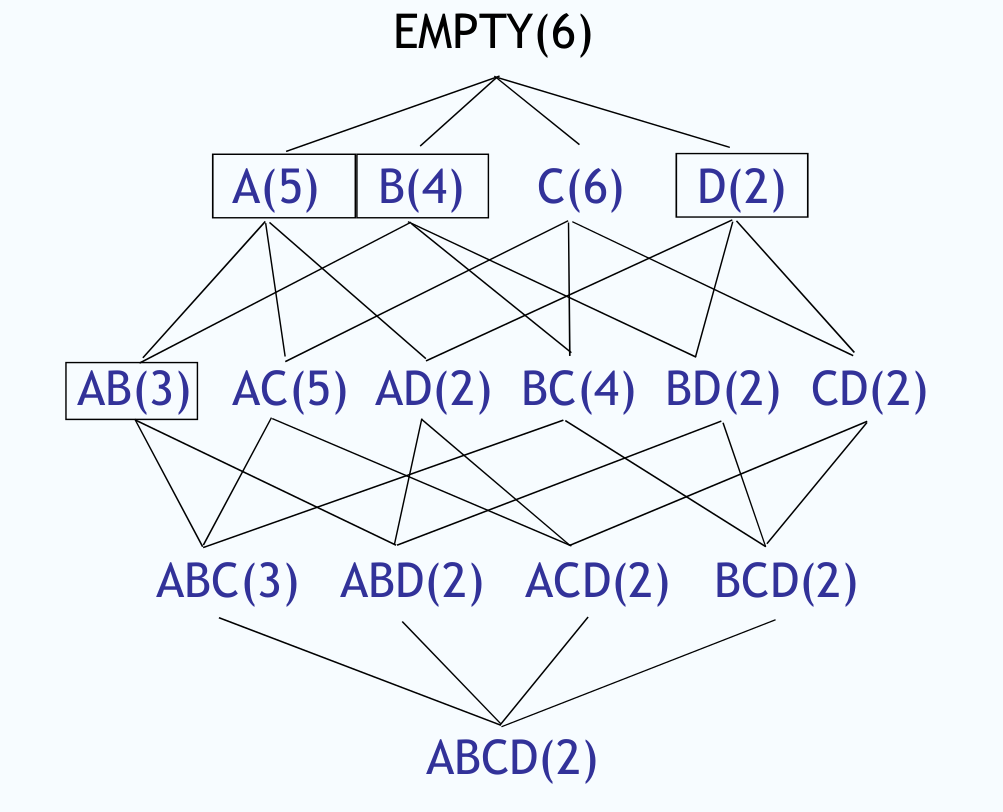
\includegraphics[height=5cm]{pictures/free_sets.png}
\end{frame}

\begin{frame}
	\begin{itemize}			
		\item Closed-Sets: Alle nachfolgenden Sets müssen weniger häufiger sein
		\begin{itemize}
			\item Füge am Anfang alle einelementige freq-Tupel zur Lösung hinzu
			\item Nach jeder Iteration gehe über die freq-Tupel und lösche die dazugehörigen Subtupel aus der Lösung, die gleich häufig sind
		\end{itemize}
	\end{itemize}
		\centering
		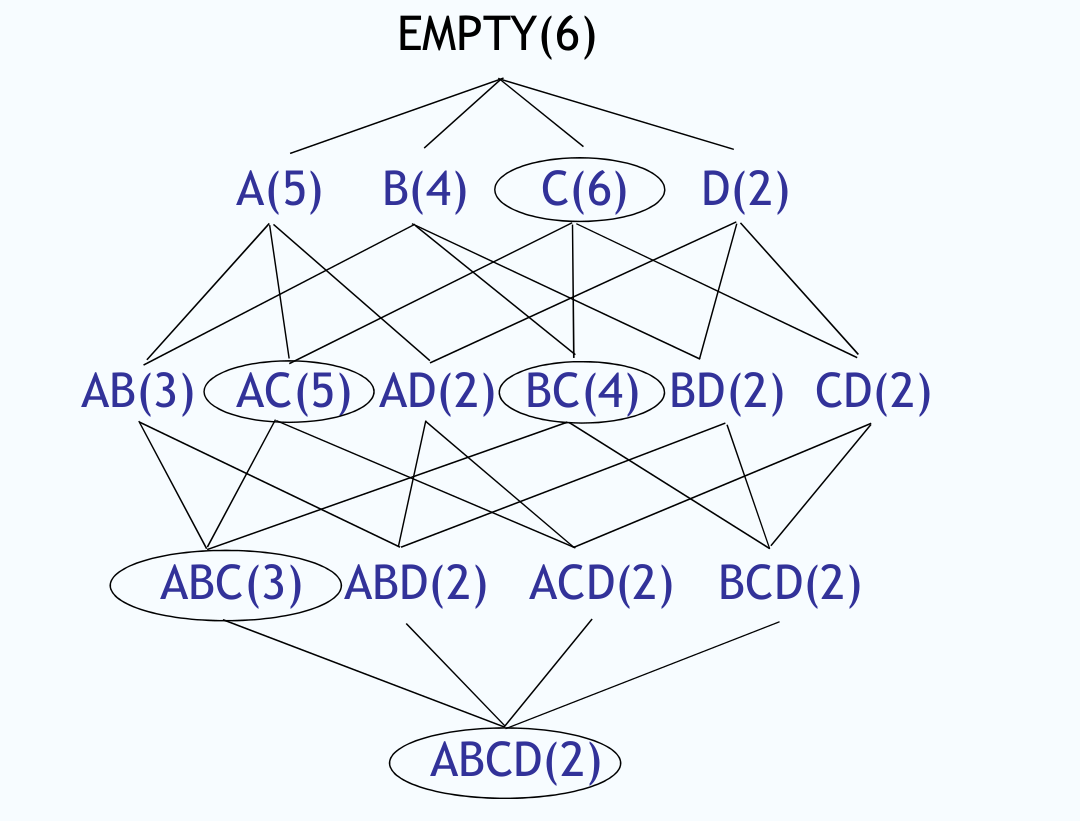
\includegraphics[height=4.5cm]{pictures/closed_sets.png}
\end{frame}

\section{Code}
\begin{frame} %%Eine Folie
	\frametitle{Code} %%Folientitel
\end{frame}






\section{Runtimes}
\begin{frame} %%Eine Folie
	\frametitle{Runtimes ohne Berechnung der Borders und Sets} %%Folientitel
	\begin{table}    
		\centering    
		\begin{tabular}{|c|c|c|c|c|c|c|}    
			\hline file \textbackslash threshold& 0.4& 0.5& 0.6& 0.7& 0.8& 0.9\\
			\hline dm1& 5,860& 9,220& 8,799& 7,960& 7,270& 6,499\\
			\hline dm2& 8,300& 9,790& 9,769& 6,669& 9,790& 6,369\\
			\hline dm3& 119,750& 9,280& 19,299& 7,730& 10,140& 11,339\\
			\hline dm4& 23431& 5249& 1878& 859,5& 597,7& 341,1\\
			\hline 
		\end{tabular}    
		\caption{alle Zeiten in $*10^{-4}s$}    
	\end{table}    
\end{frame}

\begin{frame} %%Eine Folie
	\frametitle{Runtimes mit Berechnung Borders und Sets} %%Folientitel
	\begin{table}    
		\centering    
		\begin{tabular}{|c|c|c|c|c|c|c|}    
			\hline file\textbackslash threshold& 0.4& 0.5& 0.6& 0.7& 0.8& 0.9 \\
			\hline dm1& 2,636& 1,790& 1,668& 1,492& 1,425& 1,201\\
			\hline dm2& 1,688& 1,306& 1,153& 1,172& 1,192& 1,157\\
			\hline dm3& 11,58& 5,757& 4,318& 2,939& 1,916& 1,263\\
			\hline dm4& 11669 & 2145& 289,903& 71,260& 31,589& 21,732\\
			\hline 
		\end{tabular}    
		\caption{alle Zeiten in $*10^{-3}s$}    
	\end{table}    
\end{frame}













\end{document}